	\documentclass[12pt,a4paper,italian]{article}


\usepackage[italian]{babel}
\usepackage[latin1]{inputenc}
\usepackage{amsmath}
\usepackage{amsfonts}
\usepackage{amssymb}
\usepackage{color}
\usepackage{xcolor}
\usepackage{hyperref}
\usepackage[all]{hypcap}
\usepackage{ifthen}
\usepackage{wrapfig}
%\author{Piero Bizzotto}
\usepackage[top=2cm,bottom=5cm,left=80pt,right=80pt]{geometry}
\usepackage{graphicx}
\DeclareGraphicsExtensions{.jpg,.png}

\newcommand{\ajax}{AJAXDRAW}
\newcommand{\sito}{\href{http://ajaxdraw.sourceforge.net}{http://ajaxdraw.sourceforge.net}}

\setlength{\parindent}{0pt} %settato indentazione di default 
\setlength{\headheight}{3cm} %settato grandezza header...in altre parole, quanto distanzio il doc dall'intestazione

\usepackage{fancyhdr} %pacchetto per le intestazioni
\pagestyle{fancy} %uso del pacchetto


\fancyhead{} %annulla head di default
\fancyfoot{} %annulla foot di default


\usepackage{lastpage} %setto pg di pgtot a rfoot
     \rfoot{pagina \thepage\ di \pageref{LastPage}}


\lfoot{Versione: \insertversion} %setto versione doc a lfoot
\renewcommand{\footrulewidth}{0.5pt} %ridefinisco il valore della riga di intestazione
\renewcommand{\headrulewidth}{0.5pt} %ridefinisco il valore della riga di pie' di pagina

\newcommand{\insertversion}{0.0} %definisco il nuovo comando per inserire la versione


\lhead{  \begin{Huge} \ajax \end{Huge} \\  %intestazione di sinistra
					%\begin{Large}	Software per il Disegno Grafico\\ in Tecnologie Web \end{Large}  
					\begin{normalsize}\sito \end{normalsize}
			%\\ versione documento: \insertversion\ del \today} %setto l'intestazione sx
		}
\rhead{ %includo logo nell'intestazione dx
	 	
\includegraphics[scale=0.5]{../logo/logo}  
}


%CREAZIONE ELENCHI NUMERATI PERSONALIZZATI
\newcounter{Lcount}
\newcounter{Rcount}
\setcounter{Lcount}{0}
\setcounter{Rcount}{0}

\newenvironment{elenconumerato}[2][ ]
{
  \begin{list}{#1\arabic{Lcount}.}
    {
	\setcounter{Rcount}{\value{Lcount}}
	\setcounter{Lcount}{0} 
	\usecounter{Lcount} 
\addtolength{\leftmargin}{#2pt}
	}
}
{
  \end{list}
 \setcounter{Lcount}{\value{Rcount}}
}

%CREAZIONE ELENCHI PUNTATI
\newenvironment{elencopuntato}[1][]
{
\begin{list}{\textbullet} %\itemindent=#1pt
	{
	\addtolength{\leftmargin}{#1pt}
	}
} 
{
\end{list}
}


\newenvironment{elencodescrittivo}[1][]{\begin{description} \setlength{\itemindent}{#1pt} \addtolength{\leftmargin}{#1pt}} {\end{description}}

\newcommand{\TITOLODOC}{Titolo}

%footer centrale
\cfoot{ \TITOLODOC \\  E-mail:    \href{ mailto:webshape.contact@gmail.com}{ webshape.contact@gmail.com}  }

%INSERIMENTO IMMAGINI
\newcommand{\imagerealsize}[1]{\vspace{20pt} \includegraphics{#1} }
\newcommand{\imageadapted}[1]{\vspace{20pt} \includegraphics[width=1\textwidth]{#1} }

\newcommand{\glosspath}{.\glossario}
\newcommand{\gloss}[1]{\hyperref{\glosspath~\glossario.pdf}{}{#1}{#1}}

\hypersetup{
    %bookmarks=true,         % show bookmarks bar?
    %unicode=false,          % non-Latin characters in Acrobat’s bookmarks
	%pdftoolbar=true,        % show Acrobat’s toolbar?
	%pdfmenubar=true,        % show Acrobat’s menu?
    %pdffitwindow=true,      % page fit to window when opened
    %pdftitle={My title},    % title
    %pdfauthor={Author},     % author
    %pdfsubject={Subject},   % subject of the document
    %pdfnewwindow=true,      % links in new window
    %pdfkeywords={keywords}, % list of keywords
    colorlinks=true,         % false: boxed links; true: colored links
    linkcolor=black,           % color of internal links
    %citecolor=green,        % color of links to bibliography
    %filecolor=magenta,      % color of file links
    urlcolor=teal    % color of external links
%	linktocpage=false;
}


%COLORAZIONE TESTO
\newcommand{\blue}[1]{{\color {blue} #1}} 
\newcommand{\red}[1]{{\color {red} #1}}
\newcommand{\green}[1]{{\color {green} #1}}
\newcommand{\sezione}[1]{\leftskip=0pt \section{#1} \leftskip=18pt}
\newcommand{\subsezione}[1]{\leftskip=18pt \subsection{#1} \leftskip=36pt}
\newcommand{\subsubsezione}[1]{\leftskip=36pt \subsubsection{#1} \leftskip=54pt}
\newcommand{\subsubsecindent}{54}
\newcommand{\subsecindent}{36}
\newcommand{\secindent}{18}
\newcommand{\normindent}{8}
\newcommand{\code}[1]{{\bfseries \texttt{#1}}}
\newcommand{\paragrafo}[1]{\leftskip=36pt \paragraph{#1} \leftskip=54pt}
\newcommand{\subparagrafo}[1]{\leftskip=54pt \subparagraph{#1} \leftskip=72pt} %BASE!!!

\title{\TITOLODOC}
\author{Dal Bosco Davide}

\begin{document}

\renewcommand{\insertversion}{0.2} %INSERIRE LA VERSIONE QUI DENTRO STILE x.x.xx
\renewcommand{\TITOLODOC}{Piano di Progetto} %INSERIRE IL TITOLO DEL DOCUMENTO DA FAR COMPARIRE A PIE PAGINA
\renewcommand{\glosspath}{.\glossario} %INSERIRE PERCORSO RELATIVO

%%%%%%%%%%%%%%%%%%%%%%PARTE DA NON MODIFICARE%%%%%%%%%%%%%%%%%
\begin{titlepage}
\begin{center}
	\begin{Large}	\today \end{Large}
\end{center}

\vspace{20pt}

\begin{center}
	\begin{Huge}
				\textbf{\ajax}
	\end{Huge}
\end{center}			

\begin{center}
	\begin{large}
				\textbf{Software per il Disegno Grafico in Tecnologie Web}
	\end{large}
\end{center}			

\vspace{20pt}

\begin{center}

\includegraphics[width=150pt]{../logo/logo}
\end{center}

\vspace{170pt}
\begin{center} %INSERIRE ALL'INTERNO IL TITOLO DOCUMENTO CHE COMPARIRA NELLA PAGINA INIZIALE				
	\begin{Huge}
				\textbf{\TITOLODOC}
	\end{Huge}
			\\
\end{center}
\vspace{210pt}
\begin{center}
Versione: \insertversion
\end{center}
\end{titlepage}

\newpage
%%%%%%%%%%%%%%%%%%%%%%FINE PARTE DA NON MODIFICARE%%%%%%%%%%%%%%%%%

\begin{center} %INSERIRE ALL'INTERNO IL TITOLO DOCUMENTO CHE COMPARIRA NELLA PAGINA INIZIALE
	\begin{Huge}	
				\textbf{\TITOLODOC}
			\\
	\end{Huge}
\end{center}

%\setlength{\parindent}{18pt} %settato indentazione di default 
\section*{\Large Sommario:}
Il presente documento descrive l'anailisi dei costi e delle risorse effettuata dall'azienda WebShape per lo sviluppo del Capitolato C04.

 %SEZIONE SOMMARIO
\indent \indent

\section*{\Large Stato del documento:}
\indent \indent
	Formale Esterno

\section*{\Large Redazione:}
	\begin{elencopuntato}[\normindent]
		\item[-] Dal Bosco Davide
		\item[-] Cunico Marco
	\end{elencopuntato}

\section*{\Large Approvazione:}
	\begin{elencopuntato}[\normindent]
		\item Approvatore N. 1
		\item Approvatore N. 2
		\item Approvatore N. 3
	\end{elencopuntato}

\section*{\LARGE Lista di Distribuzione:}

	\begin{elenconumerato}{\normindent}
		\item WebShape \footnote{Il termine WebShape designa una collettivit\`a di individui come da organigramma contenuto nel piano di progetto fornito in allegato al presente documento}
		\item I committenti Vardanega Tullio e Conte Renato in rappresentanza \\  dell'azienda proponente Zucchetti SPA
		%\item Il committente Conte Renato
	\end{elenconumerato}

\newpage



\section*{\Large Registro delle Modifiche:}


\begin{center}
	\begin{table}[h]
		  \begin{tabular*}
			{1\textwidth}%
				{@{\extracolsep{\fill}}|p{0.1\textwidth}|p{0.54\textwidth}|p{0.26\textwidth}|}
			 \hline
%%%%%%%%%%%%%%INTESTAZIONE COLONNE%%%%%%%%%%%%%%%%%%%%%%%%%%%%%%%%%%%%%%%%%%%%%%%%%%%%%%%%%%%%%%
			\textbf{Versione}  & \textbf{Descrizione} & \textbf{Autore} \\
%%%%%%%%%%%%%%FINE INTESTAZIONE COLONNE%%%%%%%%%%%%%%%%%%%%%%%%%%%%%%%%%%%%%%%%%%%%%%%%%%%%%%%%%%%%%%
		 \hline
%%%%%%%%%%% PARTE DA MODIFICARE %%%%%%%%%%%%%%%%%%%%%%%%%%%%%%%%%%%%%%%%%%%%%%%%%%%%%%%%%%%%%%%%%		
    	  0.2 & 01/12/2008 Inserimento capitoli Introduzione,Organigramma,Pianificazione(inizio) & Dal Bosco Davide \\
    	  0.1 & 25/11/2008 Adattamento al template scelto & Dal Bosco Davide \\
    	  0.0 & 22/11/2008 Bozza iniziale & Dal Bosco Davide \\

		\hline %%FINE RIGA
%%%%%%%%%%% FINE PARTE DA MODIFICARE %%%%%%%%%%%%%%%%%%%%%%%%%%%%%%%%%%%%%%%%%%%%%%%%%%%%%%%%%%%
		\end{tabular*}
	\caption{didascalia tabella 	MODIFICHE} %INSERIRE DIDASCALIA - SE NECESSARIA - 
	\label{tab:modifiche}
	\end{table}
\end{center}


\newpage
\thispagestyle{fancy}
\tableofcontents
\thispagestyle{fancy}
\newpage

\sezione{Introduzione}

\subsezione{Scopo del documento}
Il documento si propone di presentare ai Committenti le scelte effettuate riguardanti la distribuzione dei ruoli e delle risorse, l'assegnazione delle attivit\`a dei componenti dell'azienda e lo studio dei costi necessari per la realizzazione del progetto inerente al capitolato d'appalto C04.\\

\sezione{Organigramma}
In data 15 ottobre 2008 \`e stato costituito il gruppo WebShape formato da sei membri, tutti in possesso delle idoneit\`a necessarie per partecipare al progetto di Ingegneria del Software.
I ruoli saranno assegnati a rotazione nell'arco dello sviluppo del progetto, in base alle capacit\`a e alle disponibilit\`a dei componenti del gruppo.\\

\subsezione{Accettazione}
\begin{table}[h]
	\begin{center}
		  \begin{tabular}{|p{0.3\textwidth}|l|p{0.3\textwidth}|}
		 \hline 
		 \textbf{Cognome e Nome} & \textbf{Data} & \textbf{Firma}\\
		 \hline
		Bizzotto Piero & 15-10-2008 & \\
		Carollo Mirko & 15-10-2008 & \\
		Cunico Marco & 15-10-2008 & \\
		Dal Bosco Davide & 15-10-2008 & \\
		Dissegna Stefano & 15-10-2008 & \\
		Geremia Mirco & 15-10-2008 & \\
		\hline
		\end{tabular}
	\caption{Accettazione} 
	\label{tabella_accettazione}
	\end{center}	
\end{table}



\subsezione{Descrizione Componenti}
Vedere Tabella: (\ref{tab:tabella_componenti}) della pagina ~\pageref{tab:tabella_componenti}\\

\subsezione{Assunzioni Iniziali}
Regole da rispettare per la realizzazione del progetto didattico:
\begin{elenconumerato}{\normindent}
				\item Importo complessivo (da inserire).\\
				\item Numero totale di ore dedicate alla realizzazione del progetto (da inserire).\\
				\item L'impegno individuale di ogni componente varia da un minimo di 85 ore ad un massimo di 105 ore.\\
			\end{elenconumerato}

\begin{table}[h]
	\begin{center}
		  \begin{tabular}{|p{0.3\textwidth}|l|l|}
		 \hline 
		 \textbf{Cognome e Nome} & \textbf{Matricola} & \textbf{E-mail}\\
		 \hline
		Bizzotto Piero & 540804 & piero.bizzotto@gmail.com \\
		Carollo Mirko & 542902 & da definire\\
		Cunico Marco & 540754 & marco.cunico@gmail.com\\
		Dal Bosco Davide & 539402 & mrdavi86@gmail.com\\
		Dissegna Stefano & 561011 & stefano.dissegna@gmail.com \\
		Geremia Mirco & 563665 & crittico@gmail.com\\
		\hline
		\end{tabular}
	\caption{Descrizione dei Componenti} 
	\label{tab:tabella_componenti}
	\end{center}	
\end{table}



\subsezione{Attribuzione dei Ruoli}
Date le Assunzioni Iniziali precedentemente descritte, ed essendo il gruppo WebShape costituito da sei membri, si avr\`a una media di circa 105 ore di lavoro per persona. La durata complessiva del progetto sar\`a di circa ? ore, ogni componente lavorer\`a quindi una media di 2,5 ore giornaliere. Sono previste altre 3 revisioni:
\begin{elenconumerato}{\normindent}
				\item Revisione di Progetto Preliminare (RPP)
				\item Revisione di Qualifica (RQ)
				\item Revisione di Accettazione (RA)
			\end{elenconumerato}
La rotazione dei ruoli avviene come da tabella ?. Dato che ogni componente del gruppo dovr\`a assumere tutti i ruoli,\`e previsto che nelle varie fasi del progetto i membri della societ\`a si assumano piu' incarichi. Non \`e permesso che uno stesso membro ricopra ruoli in conflitto di interessi tra loro.\\

\sezione{Pianificazione}
Per la realizzazione del progetto l'azienda WebShape ha valutato con attenzione i possibili modelli di cicli di vita da utilizzare, tenendo conto di eventuali pregi e difetti. 
La scelta \`e ricaduta sul modello incrementale, in quanto, vista la tipologia modulare del progetto, si adatta meglio alle nostre esigenze. Con il modello incrementale abbiamo la possibilit\`a di effettuare dei rilasci di versioni parziali in modo da avvicinarci incrementalmente al prodotto finale ed effettuare una pianificazione ben definita, che sono dei vantaggi importanti per una nuova azienda. Sono stati invece scartati gli altri modelli: il modello sequenziale perch\`e \`e troppo orientato ai documenti e per il fatto che il primo prodotto del progetto si vede solo al termine della Fase di Qualifica, il modello evolutivo per la necessit\`a di un costante rilascio di versioni e il modello a spirale per l'esigenza di avere continui contatti col cliente.\\
\subsezione{Ore e costi totali}
In questa sottosezione presenteremo il nostro preventivo totale, comprendente i costi e le ore stimate, necessarie per la realizzazione del progetto. Il preventivo tiene conto di tutte le fasi di progettazione sostenute dall'Azienda.

\begin{table}[h]
	\begin{center}
		  \begin{tabular}{|c|c|c|c|}
		 \hline 
		 \textbf{Ruolo} & \textbf{Ore di lavoro} & \textbf{Costo in euro}\\
		 \hline
		Responsabile & 89 & 2670 \\
		Amministratore & 94 & 1880\\
		Analista & 45 & 1125\\
		Progettista & 150 & 3300\\
		Programmtore & 90 & 1440 \\
		Verificatore & 162 & 2592\\
        \hline
        \textbf{Totale} & \textbf{630} & \textbf{13007}\\
		\hline
		\end{tabular}
	\caption{Preventivo totale} 
	\label{tab:tabella_preventivo}
	\end{center}	
\end{table}

\begin{center}
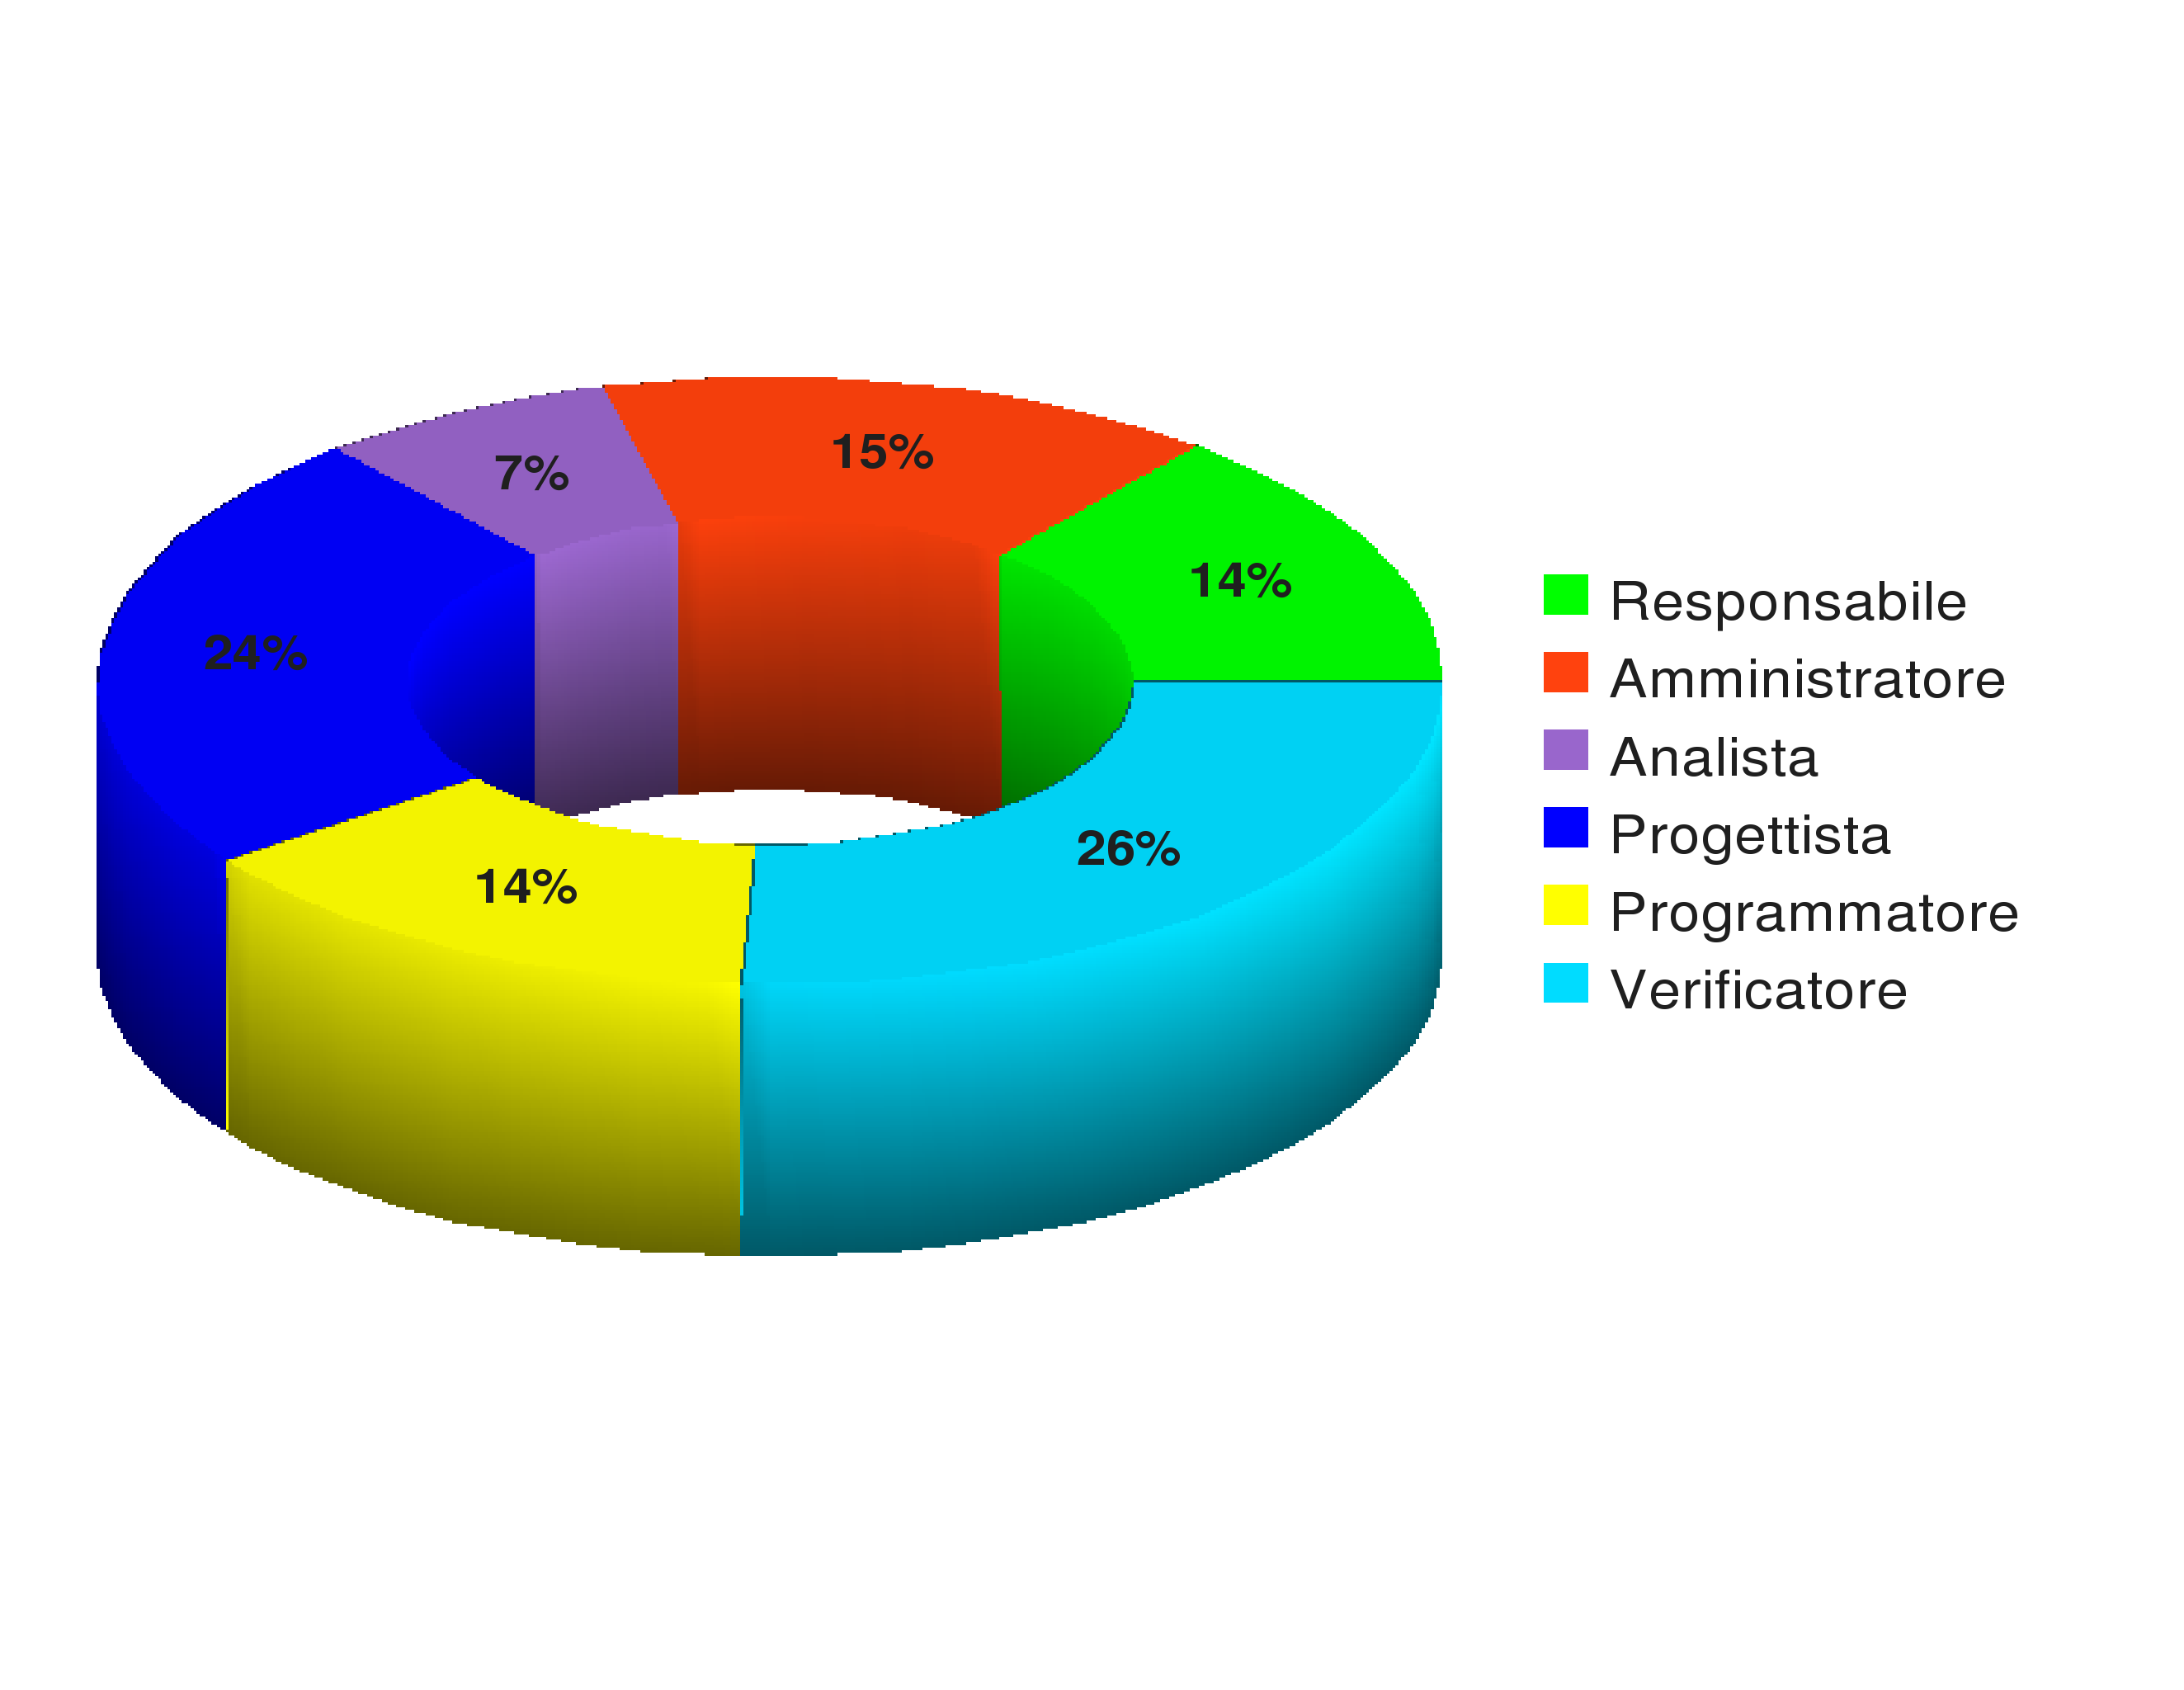
\includegraphics[width=300pt]{grafico}
\end{center}


da completare\\
\subsezione{Pianificazione economico-temporale RR-RPP}
da completare\\
\subsezione{Pianificazione economico-temporale RPP-RQ}
\begin{figure}[!ht]
\centering
\vspace{20pt} 
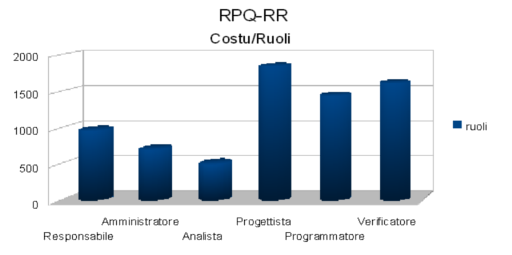
\includegraphics{RPP-RQ}
\caption{RPP-RQ: costi/ruoli}
\label{RPP-RQ}
\end{figure}

\begin{figure}[!ht]
\centering
\vspace{20pt} 
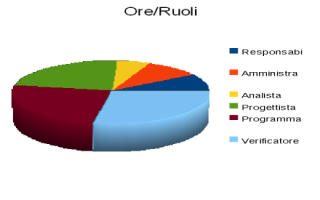
\includegraphics{RPP-RQ-torta}
\caption{RPP-RQ: ore/ruoli}
\label{RPP-RQ ore}
\end{figure}
da notare che i grafici sono una prova, infatti i nomi sono sbagliati!\\
da completare\\
\subsezione{Pianificazione economico-temporale RQ-RA}
da completare\\
\subsezione{Distribuzione dei ruoli}
da completare\\
\subsubsezione{Distribuzione per fase di progetto}
da completare\\
\subsubsezione{Distribuzione dei carichi di lavoro}
da completare\\
\sezione{Gestione del Piano di Progetto}
da completare\\
\subsezione{Obiettivi}
da completare\\
\sezione{Analisi e Gestione dei Rischi}
da completare\\

\end{document}
